\documentclass[12pt, titlepage]{article}

\usepackage{fullpage}
\usepackage[round]{natbib}
\usepackage{multirow}
\usepackage{booktabs}
\usepackage{tabularx}
\usepackage{graphicx}
\graphicspath{ {./images/} }
\usepackage{float}
\usepackage{hyperref}
\hypersetup{
    colorlinks,
    citecolor=blue,
    filecolor=black,
    linkcolor=red,
    urlcolor=blue
}

%% Comments

\usepackage{color}

\newif\ifcomments\commentstrue %displays comments
%\newif\ifcomments\commentsfalse %so that comments do not display

\ifcomments
\newcommand{\authornote}[3]{\textcolor{#1}{[#3 ---#2]}}
\newcommand{\todo}[1]{\textcolor{red}{[TODO: #1]}}
\else
\newcommand{\authornote}[3]{}
\newcommand{\todo}[1]{}
\fi

\newcommand{\wss}[1]{\authornote{blue}{SS}{#1}} 
\newcommand{\plt}[1]{\authornote{magenta}{TPLT}{#1}} %For explanation of the template
\newcommand{\an}[1]{\authornote{cyan}{Author}{#1}}

%% Common Parts

\newcommand{\progname}{Software Engineering} % PUT YOUR PROGRAM NAME HERE
\newcommand{\authname}{Team 14, Reach
\\ Aamina Hussain
\\ David Moroniti
\\ Anika Peer
\\ Deep Raj
\\ Alan Scott} % AUTHOR NAMES                  

\usepackage{hyperref}
    \hypersetup{colorlinks=true, linkcolor=blue, citecolor=blue, filecolor=blue,
                urlcolor=blue, unicode=false}
    \urlstyle{same}
                                


\newcounter{acnum}
\newcommand{\actheacnum}{AC\theacnum}
\newcommand{\acref}[1]{AC\ref{#1}}

\newcounter{ucnum}
\newcommand{\uctheucnum}{UC\theucnum}
\newcommand{\uref}[1]{UC\ref{#1}}

\newcounter{mnum}
\newcommand{\mthemnum}{M\themnum}
\newcommand{\mref}[1]{M\ref{#1}}

\begin{document}

\title{System Design for \progname{}} 
\author{\authname}
\date{\today}

\maketitle

\pagenumbering{roman}

\section{Revision History}

\begin{tabularx}{\textwidth}{p{3cm}p{2cm}X}
\toprule {\bf Date} & {\bf Version} & {\bf Notes}\\
\midrule
2024-01-17 & 1.0 & Initial version of System Design Doc\\
\bottomrule
\end{tabularx}

\newpage

\section{Reference Material}

\href{https://github.com/davimang/REACH/blob/main/docs/SRS/SRS.pdf}{SRS Documentation}\\
\href{https://github.com/davimang/REACH/blob/main/docs/HazardAnalysis/HazardAnalysis.pdf}{HA Documentation}\\
\href{https://github.com/davimang/REACH/blob/main/docs/Design/SoftArchitecture/MG.pdf}{MG Documentation}\\
\href{https://github.com/davimang/REACH/blob/design_docs/docs/Design/SoftDetailedDes/MIS.pdf}{MIS Documentation}


\subsection{Abbreviations and Acronyms}

\renewcommand{\arraystretch}{1.2}
\begin{tabular}{l l} 
  \toprule		
  \textbf{symbol} & \textbf{description}\\
  \midrule 
  SRS & Software Requirements Specification\\
  HA & Hazards Analysis\\
  MG & Module Guide\\
  MIS & Module Interface Specification\\
  \bottomrule
\end{tabular}\\

\newpage

\tableofcontents

\newpage

\listoftables

\listoffigures

\newpage

\pagenumbering{arabic}

\section{Introduction}

This document includes an overview of the system design for the web application REACH. 
REACH will provide a platform which will allow patients to have better access to clinical trials and make it 
easier for practitioners to find potential participants and match them to studies they are eligible for. 
It does this by pulling in information from existing repositories of active research studies.

\section{Purpose}

The purpose of this system design document is to provide an overview of the system for REACH. This includes the 
average behavior of the system or web application REACH, as well as how the design connects to and satisfies the 
requirements stated in the \href{https://github.com/davimang/REACH/blob/main/docs/SRS/SRS.pdf}{SRS Documentation}. 
It will also include any applicable user interface designs to help visualize how the mentioned requirements are 
being satisfied. The \href{https://github.com/davimang/REACH/blob/main/docs/Design/SoftArchitecture/MG.pdf}{MG Documentation} 
and \href{https://github.com/davimang/REACH/blob/design_docs/docs/Design/SoftDetailedDes/MIS.pdf}{MIS Documentation} 
provide further details of the software architecture and modules of the system.

\section{Scope}

The scope is documented in the \href{https://github.com/davimang/REACH/blob/main/docs/SRS/SRS.pdf}{SRS Documentation}.

\section{Project Overview}

\subsection{Normal Behaviour}

A normal user scenario for REACH would be:

\begin{enumerate}
  \item User opens the website REACH.

  \item User logs in to their account.

  \item User inputs their personal information into a profile and saves it.
  
  \item User selects the previously saved profile and inputs data about their condition.
  
  \item Reach displays a list of applicable clinical trials sorted by distance.
  
  \item User selects a trial and chooses to contact the research coordinator for the trial.
  
  \item Reach creates an email template for the user using the provided information.
  
  \item User leaves the website.
\end{enumerate}

\noindent
Other scenarios are documented in the \href{https://github.com/davimang/REACH/blob/main/docs/SRS/SRS.pdf}{SRS Documentation}

\subsection{Undesired Event Handling}

The handling of undesired events is documented in the \href{https://github.com/davimang/REACH/blob/main/docs/HazardAnalysis/HazardAnalysis.pdf}{Hazards Analysis Documentation}.

\subsection{Component Diagram}

N/A no hardware

\subsection{Connection Between Requirements and Design} \label{SecConnection}

The connection between Requirements and Design are specified in the \href{https://github.com/davimang/REACH/blob/main/docs/Design/SoftArchitecture/MG.pdf}{Module Guide Documentation}.

\section{System Variables}

N/A

\section{User Interfaces}

The following images are mockups of the user interface for REACH. 
The mockups were created using Figma and are subject to change.

\begin{figure}[H]
  \centering
  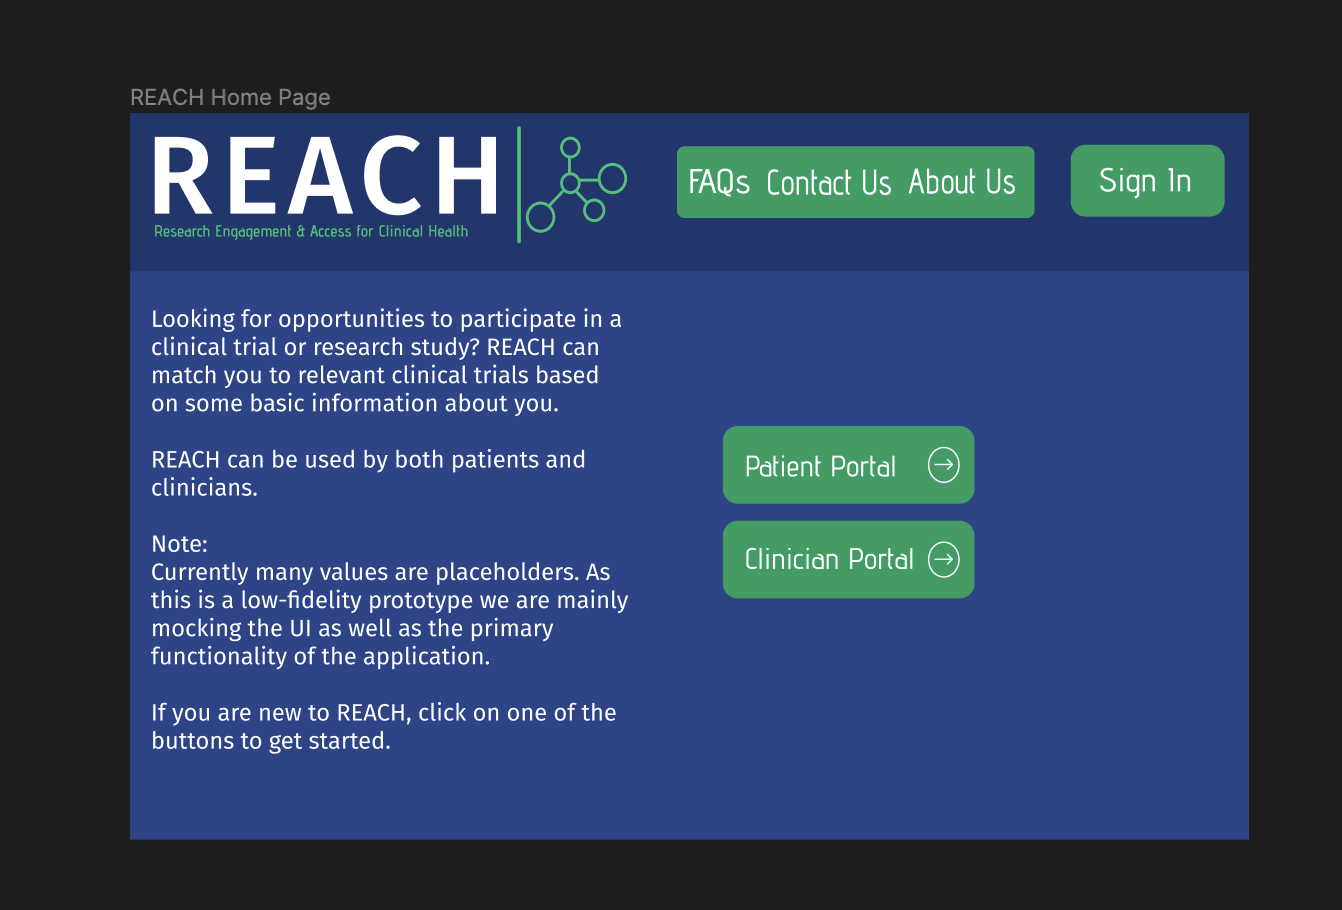
\includegraphics[width=0.9\linewidth]{images/HomePage.png}
  \caption{REACH home page}
  \label{fig:figure1}
\end{figure}
The home page allows for user input in the form of buttons allowing the linkage of 
various pages of the application. The key features on this page are the \textbf{Sign In},
\textbf{Patient Portal} and \textbf{Clinician Portal} buttons.
These are strategically placed on the right side of the page as the team expects
that users will read the text on the left side of the page first.\newline

Additionally, the buttons are in a different font as well as being
coloured bright green. This is to draw the user's attention to the buttons
while maintaining a pattern of design for the application. \newline

Given that this preliminary design is meant to act as a low-fidelity prototype, 
the team has not yet decided on the exact text that will be displayed on this page. 


\begin{figure}[H]
  \centering
  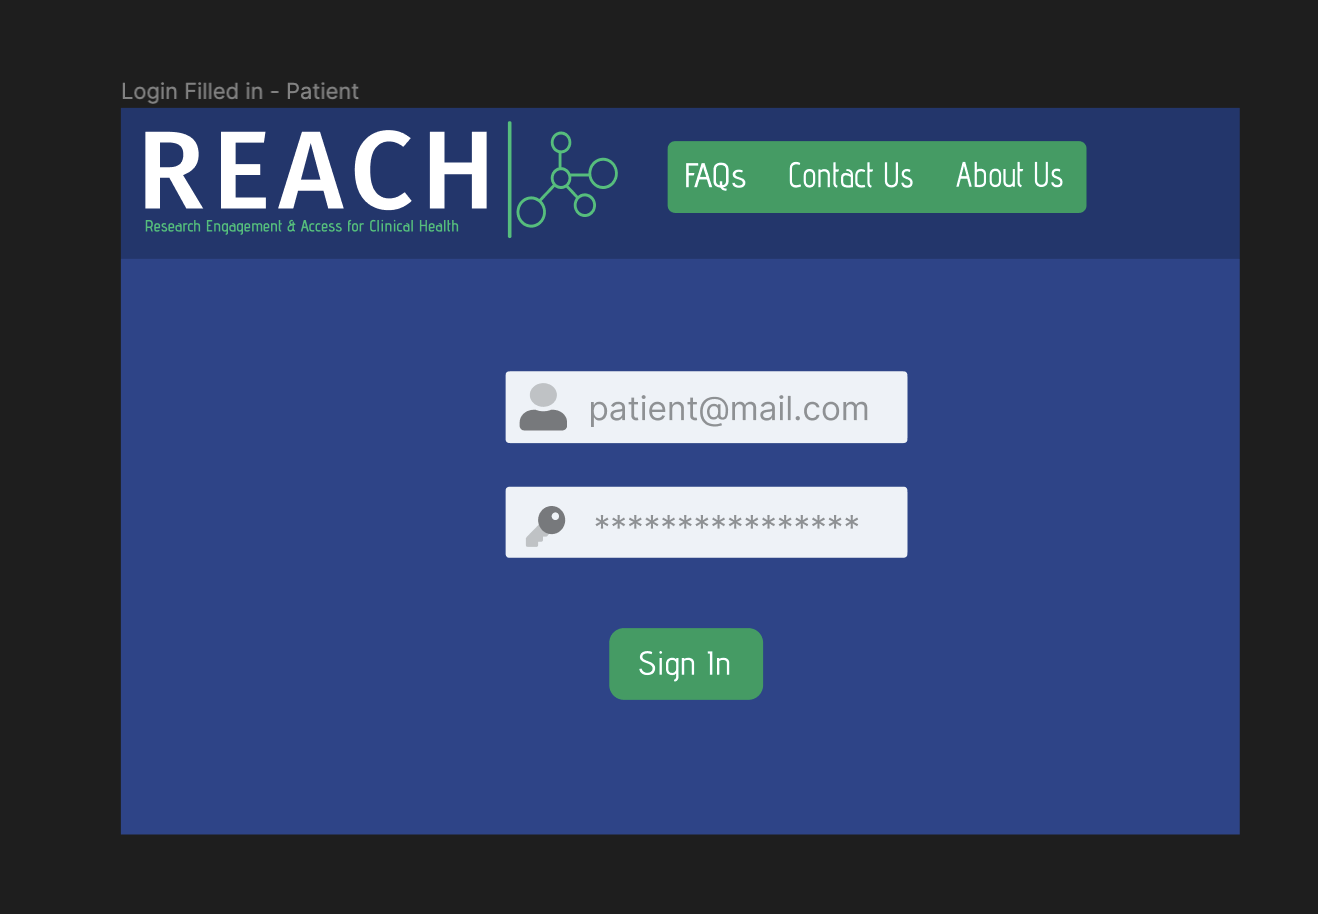
\includegraphics[width=0.9\linewidth]{images/Login.png}
  \caption{REACH login page}
  \label{fig:figure2}
\end{figure}

The login page is a simple interface with user input in the form of text fields
 as well as buttons. The text fields are for the user to input their username and password
 while the buttons are for the user to either login or visit other pages.
 As mentioned in previous sections, the design
 of the buttons is meant to capture the user's attention.

\begin{figure}[H]
  \centering
  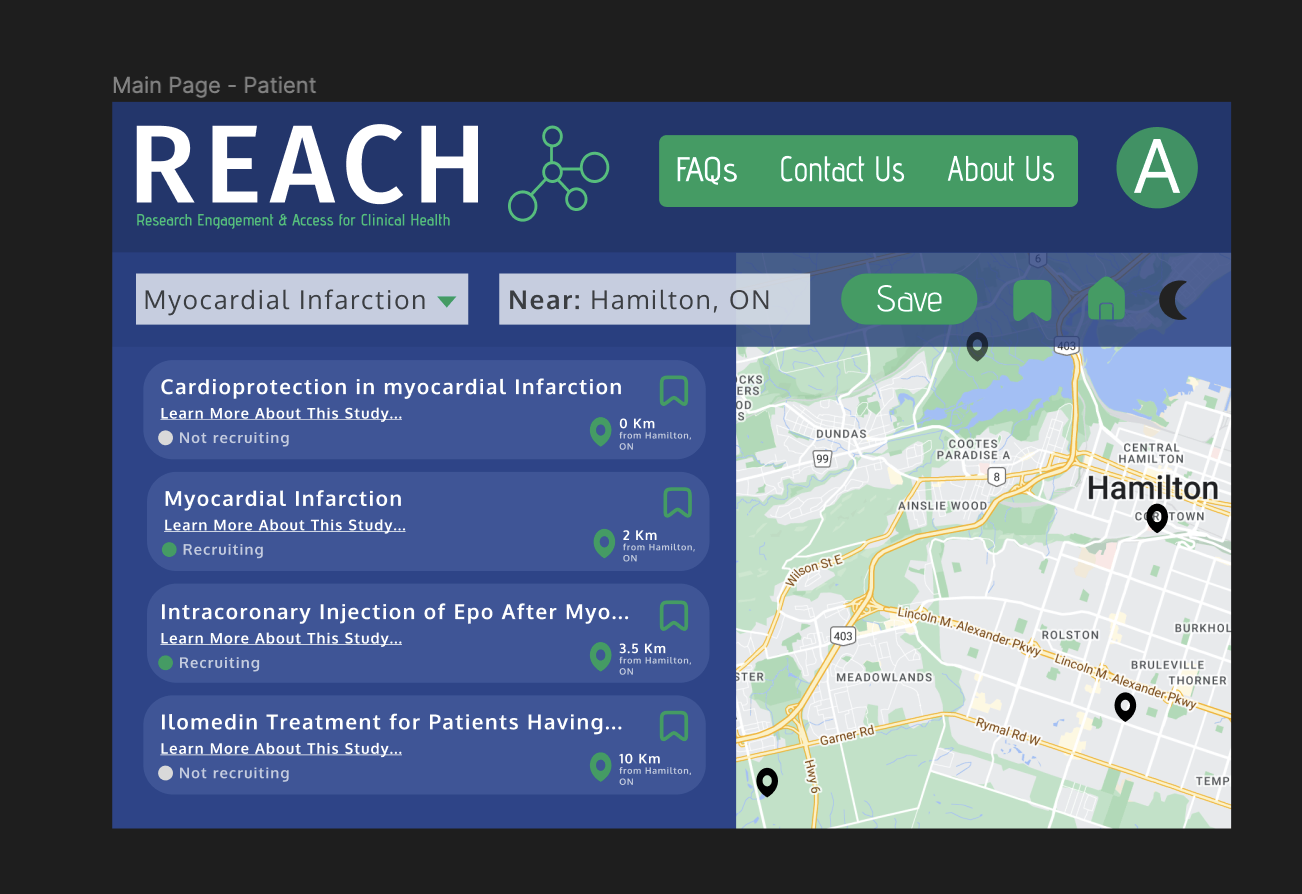
\includegraphics[width=0.9\linewidth]{images/MainPage.png}
  \caption{REACH main page with query results}
  \label{fig:figure3}
\end{figure}
The main page for the application presents the most features to the user. 
Although the final application will have more filtering
and search capabilities, the current design is a mockup of a sample search allowing the
 user to see the results as well as the scroll bar indicating further results. \newline
 
 The map on the right side of
 the screen pins locations of the nearest trials to the location the user has specified. \newline
 
 Additional buttons are present allowing the user to edit their account information, 
 save a trial to their bookmarks, save a search and return to the home page. 

\begin{figure}[H]
  \centering
  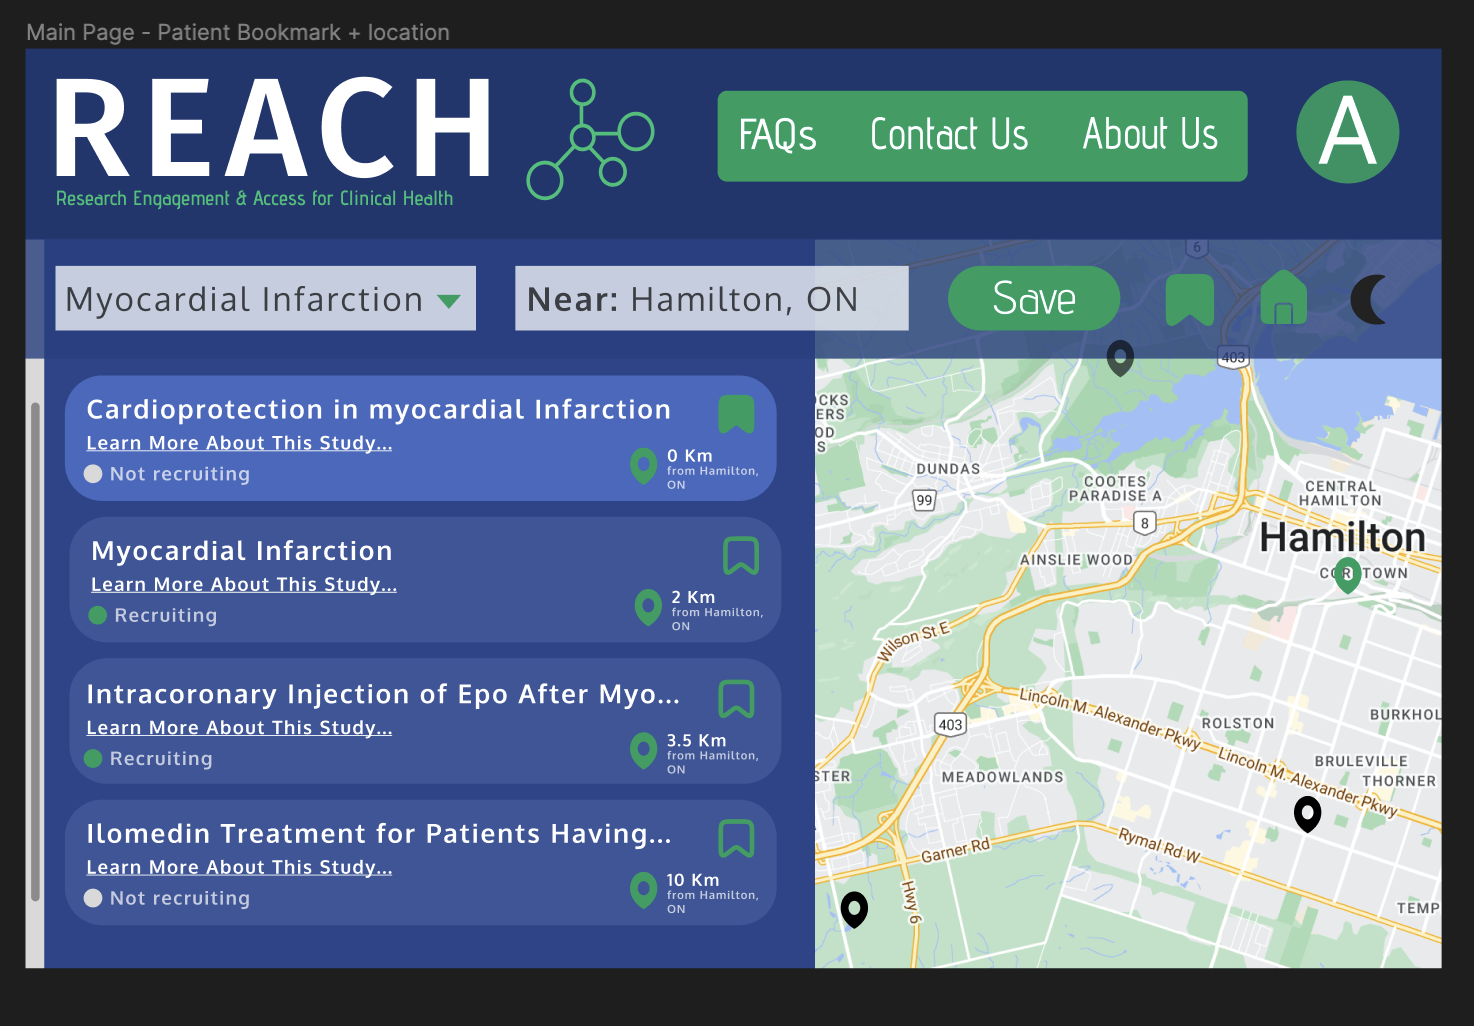
\includegraphics[width=0.9\linewidth]{images/Bookmark.png}
  \caption{REACH main page with bookmark functionality}
  \label{fig:figure4}
\end{figure}

This screen represents the bookmark functionality of the application. 
The user can bookmark a trial and it shall be saved to their account for future reference. 
The bookmark interface is the simple click of a button which results in 
the filling of the icon. \newline


To see the mockups with the interactions currently
the team is currently working on, visit the \href{https://www.figma.com/file/58wCxZa5xulKIIYw8eX8Pr/REACH-Trial-Functionality?type=design&node-id=0%3A1&mode=design&t=ff0O5TWpZokg19Q8-1}{Figma Project}.


\section{Design of Hardware}

N/A

\section{Design of Electrical Components}

N/A

\section{Design of Communication Protocols}

The communication protocol used by the application is when it is communicating with ClinicalTrials.gov.
The purpose of this external communication is to fetch trials from ClinicalTrials.gov.
This is done by utilizing the external ClinicalTrials.gov API to fetch trials. 

\section{Timeline}

\begin{table}[H]
  \begin{tabular}{|p{0.22\textwidth}|p{0.2\textwidth}|p{0.3\textwidth}|p{0.2\textwidth}|}
  \hline
  \textbf{Timeline for Development} & \textbf{Timeline for Testing} & \textbf{Modules}                                  & \textbf{Developer(s)} \\ \hline
  November 15, 2023 - January 27, 2024                    & January 22, 2024 - February 1, 2024                & Trial Data Module                                                      & David Morontini, Alan Scott                \\ \hline
  November 15, 2023 - January 27, 2024                    & January 22, 2024 - February 1, 2024                & Trial Fetching Module                                                  & David Morontini, Alan Scott                \\ \hline
  November 15, 2023 - February 1, 2024                    & January 22, 2024 - February 3, 2024                & Trial Filtering Module                                                 & Alan Scott                                 \\ \hline
  January 20, 2024 - January 27, 2024                     & January 22, 2024 - February 1, 2024                & User Data Module, Patient Info Module                                  & David Morontini, Deep Raj                  \\ \hline
  January 20, 2024 - January 27, 2024                     & January 22, 2024 - February 1, 2024                & Registration Module, Login Module                                      & Anika Peer, Deep Raj                       \\ \hline
  January 20, 2024 - February 1, 2024                     & January 22, 2024 - February 3, 2024                & Notification System Module, Email Template Module                      & Aamina Hussain, Deep Raj                   \\ \hline
  November 15, 2023 - February 4, 2024                    & January 22, 2024 - February 5, 2024                & Data Collection Module, Trial Display Module                           & Aamina Hussain, Anika Peer                 \\ \hline
  January 20, 2024 - February 4, 2024                     & January 22, 2024 - February 5, 2024                & Registration Visualization Module, User Profile Module, Base UI Module & Aamina Hussain, Anika Peer                 \\ \hline
  \end{tabular}
  \caption{\label{TimelineTable}Timeline for Development \& Testing of Modules}
  \end{table}

% \bibliographystyle {plainnat}
% \bibliography{../../../refs/References}

\newpage{}

\appendix

\section{Interface} 

N/A 

\section{Mechanical Hardware}

N/A

\section{Electrical Components}

N/A

\section{Communication Protocols}

\section{Reflection}

The information in this section will be used to evaluate the team members on the
graduate attribute of Problem Analysis and Design.  Please answer the following questions:

\begin{enumerate}
  \item What are the limitations of your solution?  Put another way, given
  unlimited resources, what could you do to make the project better? (LO\_ProbSolutions)\\

  There are a few improvements that can be made given more (or unlimited) resources. Naturally, the resources that 
  would be most valuable are time and money, so the improvements are primarily focused around limitations due to a lack of 
  one (or both) of these resources.\\

  First, while time wouldn't be an issue, due to the lack of financial resources, we are restricted in the number of notifications that 
  can be sent to our users. As a result, we made the design decision to only include an email notification system, and ignore other types 
  of notification systems, such as sending notifications via text message. With more money, the number of notifications we can send per unit time 
  would increase, and we would then be able to explore these other types of notfications. Another limitation due to financial resources
  is the number of cloud resources that can be used. In order to keep costs low, the number of resources (such as cpus, storage, etc..) must 
  be kept to a minimum. As a result, a limitation is posed on the system with respect to how many users can be using the system at one time. if we had 
  more (or unlimited) money, we could greatly increase these resources, which would allow our system to support many more users at once.\\
  
  One design limitation due to the amount of time we have to implement the system, is the decision to use one clinical trial repository as 
  opposed to several repositories. With more time, we would likely be able to design the system in a way that is suited towards using 
  multiple repositories, however, since this would greatly increase the complexity of the application, we decided to stick with the most 
  popular repository, clinicaltrials.gov. In the case of multiple repositories, more modules would be needed, and more methods would be required 
  in these modules (whereas now, we only require 2 simple trial fetching/filtering modules).

  \item Give a brief overview of other design solutions you considered.  What
  are the benefits and tradeoffs of those other designs compared with the chosen
  design?  From all the potential options, why did you select documented design?
  (LO\_Explores)\\

  There were several design solutions that we considered for both the frontend and backend components of the application.
  Beginning with the backend modules/components, one alternative design solution was for the trial interface that would be used
  to interact with the clinicaltrials.gov website. Essentially, instead of having a separate module for the trial fetcher and filterer, these 
  would be combined into one large module, which would do all the work related to trial interactions. The pros of this design (for this part 
  of the application) is that there would be only one interface/abstraction that would need to be implemented, and it would be a bit simpler to 
  implement. The main con is that it would not be very maintainable/extendable, since the module would get messy very quickly. Additionally, we 
  decided to split the modules since each module should only be hiding one secret, and in the first case, it would technically be hiding two (how the 
  trials are fetched, and how they are filtered).

  Another design solution we considered was for the frontend visualization/interface. Specifically, the interface that would allow users 
  to view the different trials that they are eligible for. Instead of having the trials displayed vertically, with the map to the right 
  of the trials, the design would be to have trials displayed vertically and horizontally across the page. When clicking on a trial 
  for more information, you would be given the location of the trial. The pros of this design is that it is easier to implement, and simplifies
  the page as a whole, which might make the user a bit more relaxed when using the system. The cons are that the user is unable to easily see where
  the trial is located when searching through the trials, which is one of the most important pieces of information the user needs. As a result of this 
  importance, we felt that the map should be included, so the user can efficiently search through the trials, using both the description
  and location on the map.

  One final design solution that we considered was for the clinician/patient relationship. The design was that a user who logged in as 
  a clinician would be able to save multiple patient profiles, and create searches based on these profiles, whereas a regular user (i.e., not a 
  clinician) would only be able to create one profile. In comparison to the current design, there are not any pros/advantages to using this design, 
  however there are a couple disadvantages. First, the relationship between the user data module and patient info module becomes more complex 
  in the case that regular users can only create one profile. Additionally, (and most importantly), it is highly likely that a regular user might 
  want to create multiple profiles, whether it be for themselves, or for their family/friends. For these two reasons, we decided it would be 
  best to design the system in a way that supports both regular users, and clinicians to be able to create and save multiple profiles.
\end{enumerate}

\end{document}